\section{Process breakdown}

\subsection{Project's twilight}

Data visualization takes up a big role in sports media.
It is a very effective means of conveying information that once were only tables and textual statistics.
Modern times have seen an explosion of such visualizations,\cite{perin} but this evolution seems to have avoided the ski world.
The three authors being fans of alpine skiing -- and still in mourning after the premature end of the 2019-2020 season --, it is only natural to have ventured in this area to contribute to the growing field.

This is why this projects explores the results of all FIS Alpine Ski World Cup results, from its inception in 1966 until today, after the shortened 2019-2020 season.

\subsubsection{Data scraping}

Getting reliable data on the World Cup results is our first goal.
The FIS website\cite{fis-website} offers all statistics needed to reach our objectives, but the absence of an API, downloadable datasets or easily \textit{scrapable} web pages forced us to find an alternative.
Ski-DB\cite{ski-db} offers a simpler web layout which was much easier to scrape.
The data has been observed and tested to be very reliable, if not identical to the official source.

\begin{table}[h]
    \centering
    \begin{tabular}{|lllll|}
        \hline
        \multicolumn{5}{|c|}{Run-specific information}\\
        \hline
        Season & Date & Venue & Country & Event\\
        \hline
        \hline
        \multicolumn{5}{|c|}{Athlete-specific information}\\
        \hline
        Rank & Name & Country & \nth{1} run time & \nth{2} run time\\
        Total time & \multicolumn{2}{l}{Time diff. to \nth{1} rank} & Ski brand & Ski-DB ID\\
        \hline
    \end{tabular}
    \caption{Information gathered for each World Cup result since 1966 (117,839 data points)}
    \label{tab:skier_race}
\end{table}

\begin{table}[h]
    \centering
    \begin{tabular}{|llll|}
        \hline
        Name & FIS ID & Birthdate & Country\\
        \multicolumn{2}{|l}{FIS competitor ID} & Profile picture & Club\\
        \hline
    \end{tabular}
    \caption{Information gathered for each skier since 1966 (3,139 athletes)}
    \label{tab:skier_profile}
\end{table}

Table \ref{tab:skier_race} shows the information we have gathered for each skier's result, while table \ref{tab:skier_profile} is more specific for each skier.
The information on the country is not redundant, since skiers may have changed nationality during the course of their careers.
The difference between the \textit{FIS ID} and the \textit{FIS competitor ID} was essential during the scraping for obscure reasons only the FIS knows; it is only kept in case of \textit{emergency}.
These two datasets, once combined, may be used to build very strong visualizations.

\begin{figure}[ht]
    \centering
    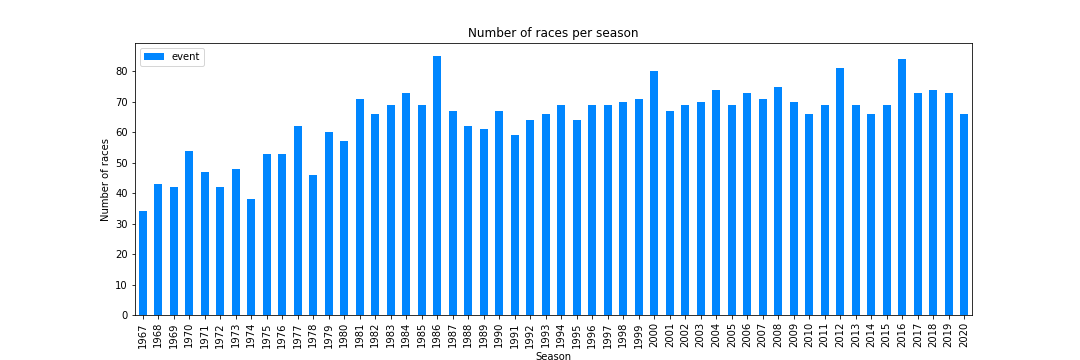
\includegraphics[width=\linewidth]{img/races_per_year.png}
    \caption{Number of races per season, period 1967-2020}
    \label{fig:races_year}
    \centering
    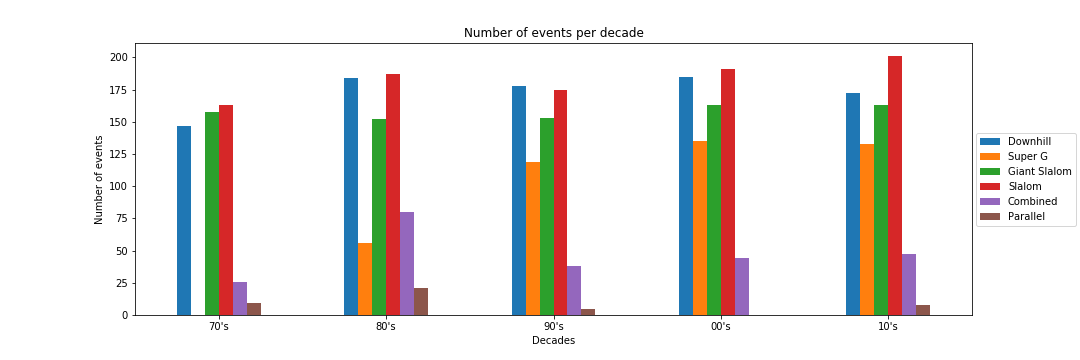
\includegraphics[width=\linewidth]{img/events_per_decades.png}
    \caption{Number of events per decade, period 1970-2019}
    \label{fig:events_decade}
\end{figure}

Figures \ref{fig:races_year} and \ref{fig:events_decade} show our early analysis efforts.
These demonstrate that there are approximately between 60 and 90 events per season since the start of the World Cup, and that types of events have also evolved to leave more room to more technical disciplines, like slalom and giant slalom.

\newpage

\subsubsection{First ideas}

Knowing the information we have at our disposal, we may now outline what exactly to visualize on a higher level.

Having such a long and detailed span of information allows us to show the results of absolutely every ski race ever.
This is not -- and should not -- be the central point of our concept since explored sources already do this, but it still has to be present in one way or another.
Another way of displaying these events is by using a map, dynamically showing the location of all the venues of a given season.

Having every World Cup result allows the creation of potentially interesting visualizations.
Past rankings are nowadays sentenced to be stored as boring text tables, reflecting absolutely nothing about the suspense and tension experienced at the time.
Dynamizing these rankings allows veteran fans to relive these moments as they happened at the time.
Race after race, event after event, month after month, the rankings will evolve and give the context to each race; for example, "why did this slalom specialist participate in a downhill event?
Oh right, it is because he is one of the main contenders of the main classification before he injured himself."
Such a scenario is not shown by a static, end-of-season ranking table.

Finally, there is a possibility of linking this gold mine of information in a completely novel way.
How do athlete compare among themselves, i.e. which skiers participate in the most varied type of events, which only stick to their specialty, etc.
This way of comparing and linking the athletes highlights the main rivalries of the time.

Figure \ref{fig:prototype} demonstrates an early idea for our website.
The structure remained the same throughout development, since it proved to be an efficient way of displaying everything.

\begin{figure}[ht!]
    \centering
    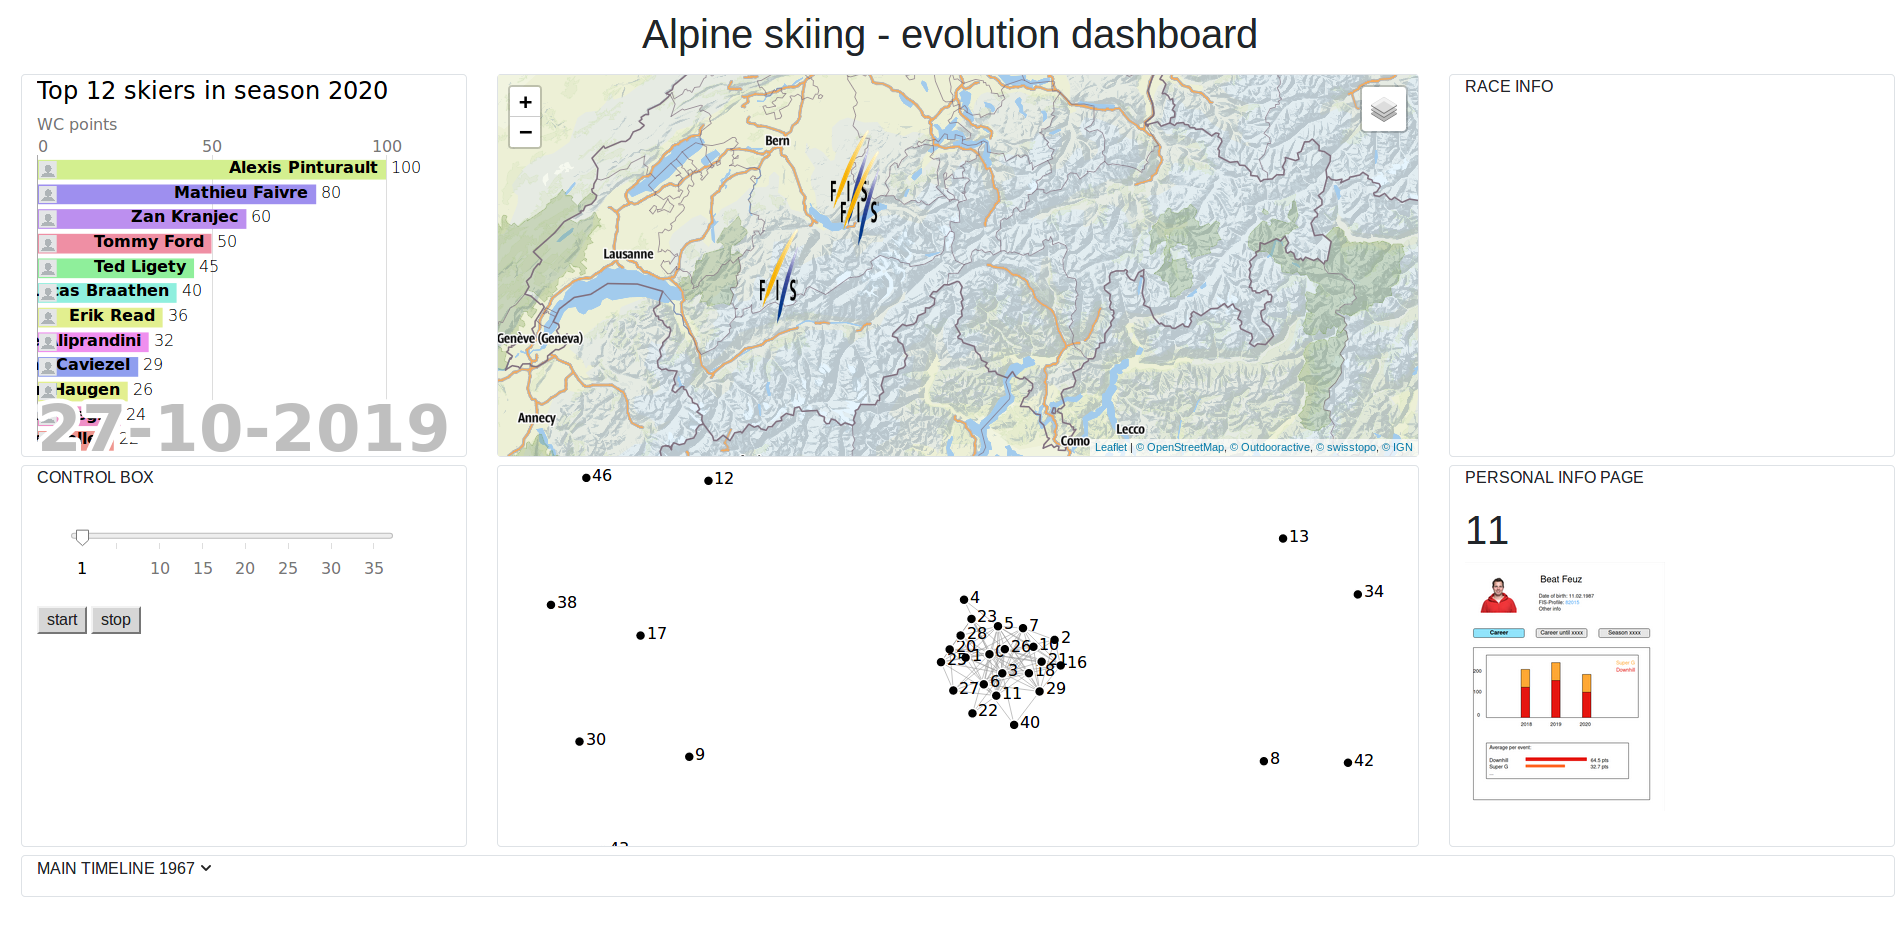
\includegraphics[width=\linewidth]{img/prototype.png}
    \caption{Early prototype of our website}
    \label{fig:prototype}
\end{figure}

\begin{figure}[ht!]
    \centering
    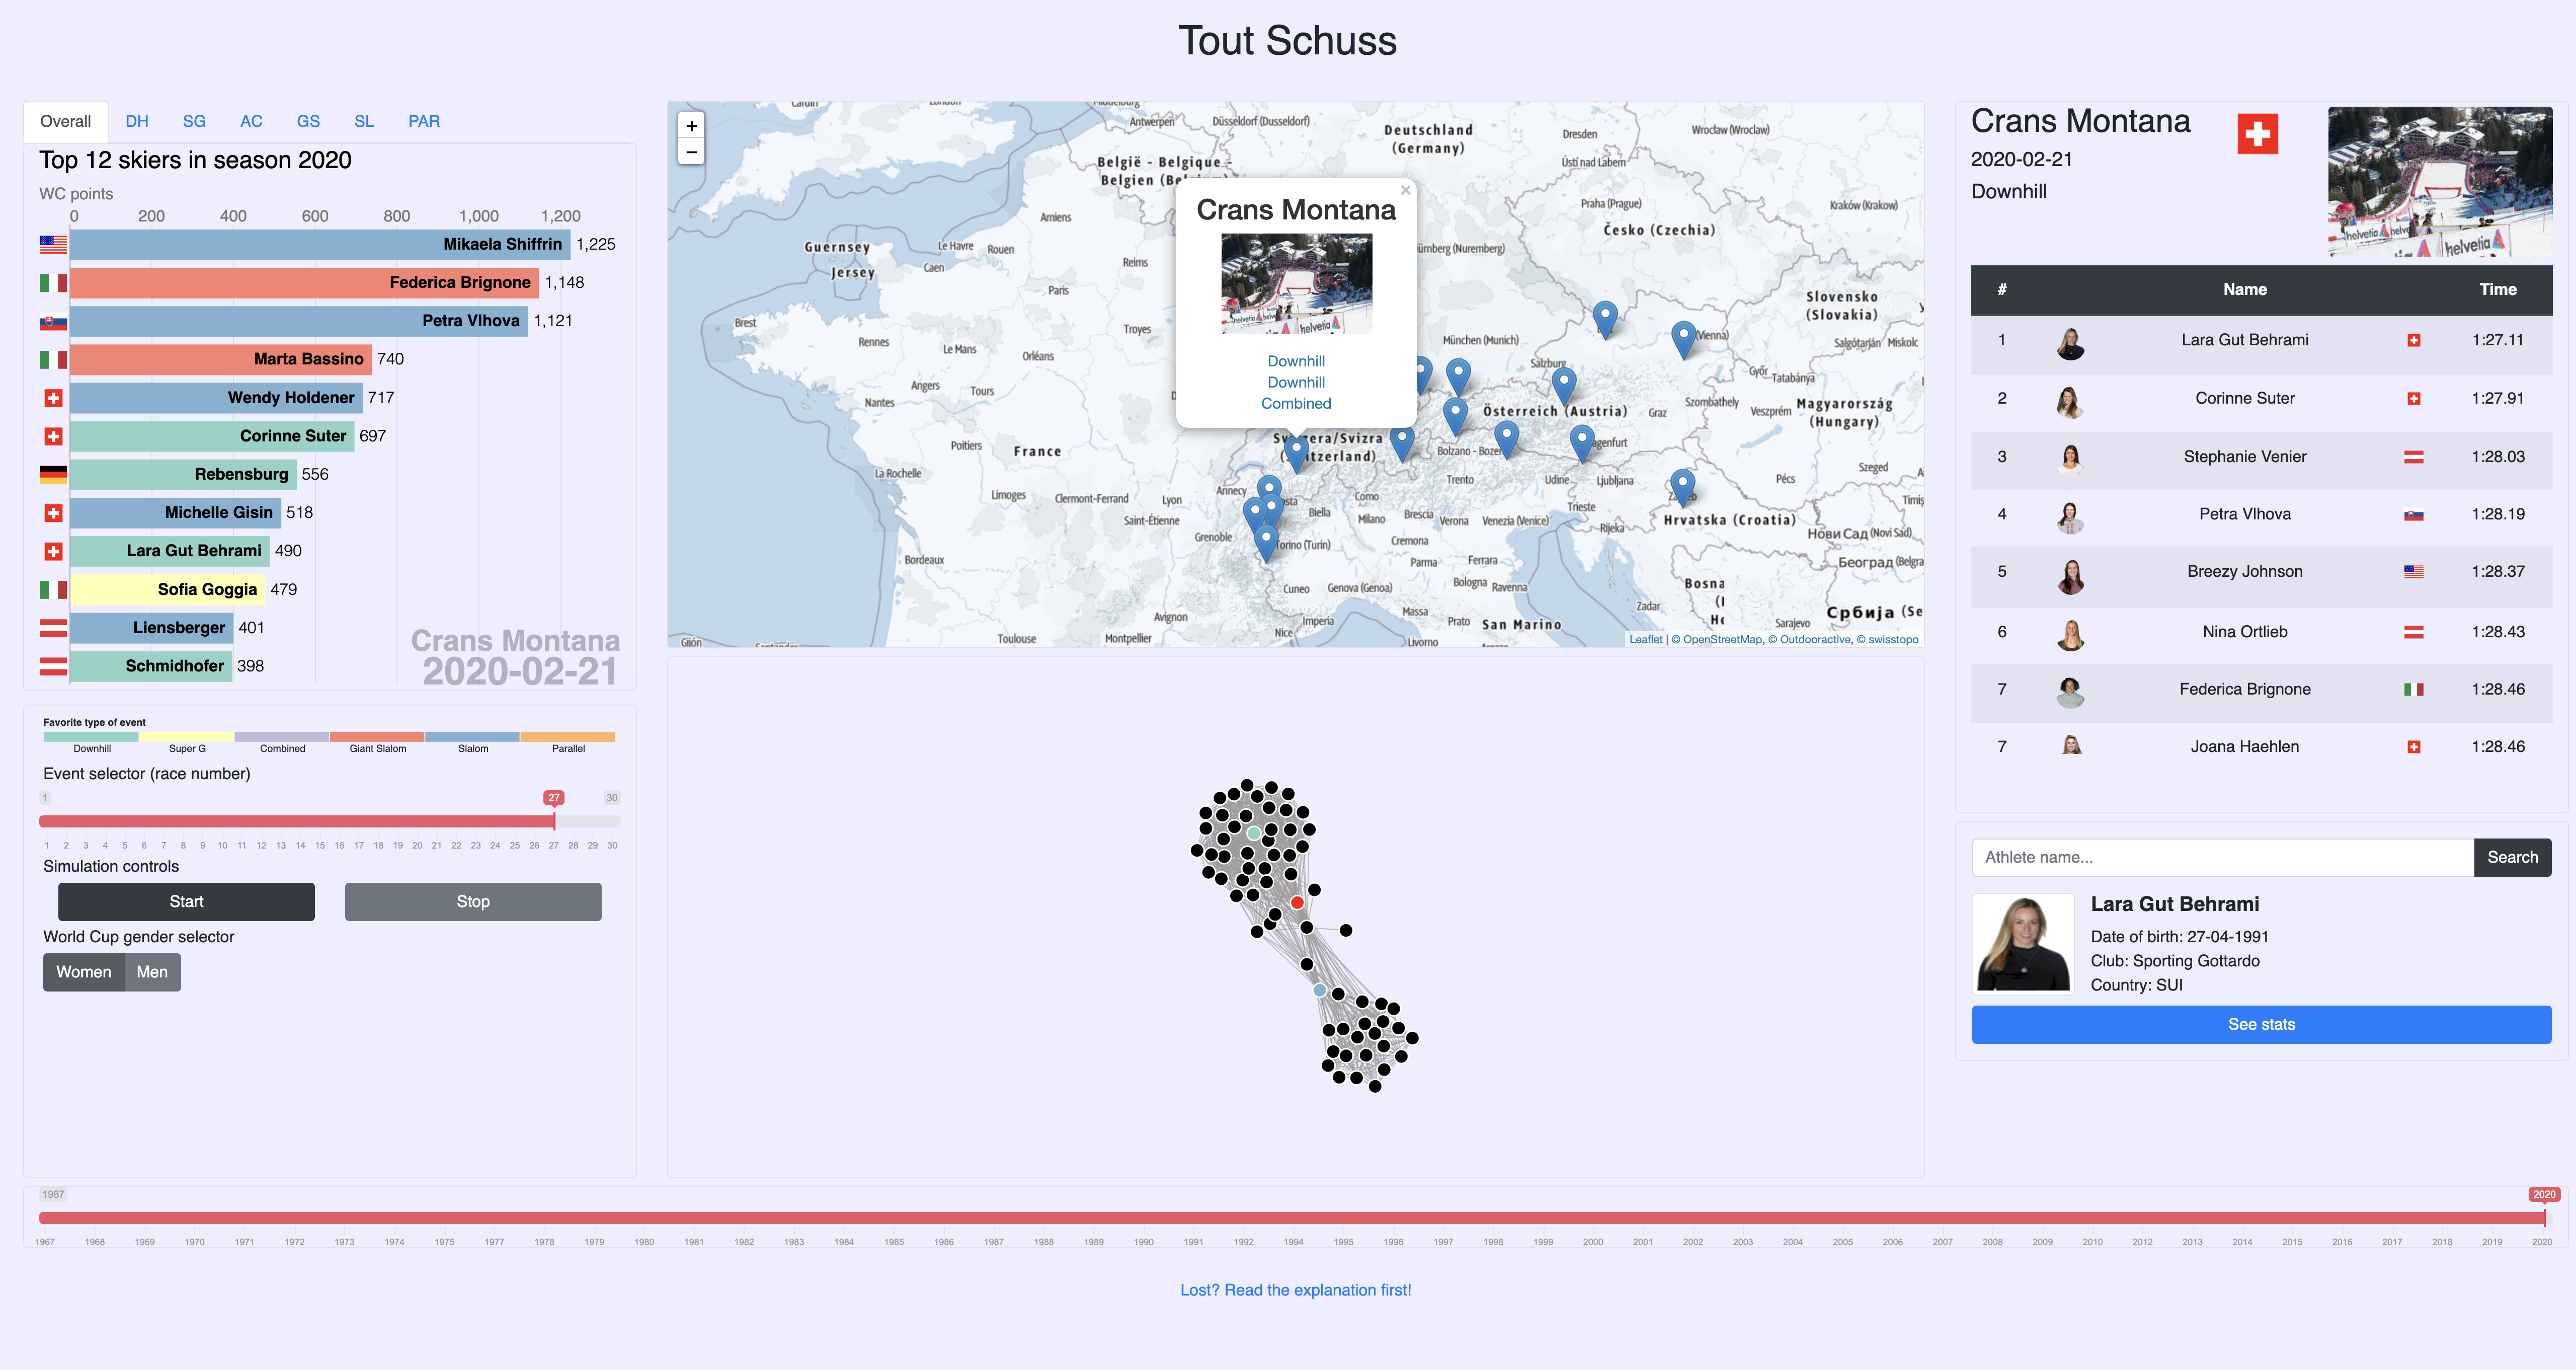
\includegraphics[width=\linewidth]{img/website.png}
    \caption{Final version of our website}
    \label{fig:final_website}
\end{figure}

\subsection{Main development}

On a high level, the user can select any season (1967-2020) and the desired gender of the competition they wish to explore -- men's or women's.
Figure \ref{fig:final_website} shows our final result, for reference.

\subsubsection{Athlete profile}
\label{sec:profile}

All skiers have a personal information page displaying their name, birth date, profile picture, club and country.
This page can be loaded by either selecting a skier in any other visualization, i.e. the graph similarity, and the bar chart race or normal race rankings.
A search bar with autocompletion is also available.
There are also different visualizations available for each skier under three different modes, either showing their whole career, their career until the \textit{selected season}, or their results of the season taking place on the \textit{selected season}.
Our data is dependent on what exists on the official FIS-website, so it is entirely possible that some information is absent or wrong for some athletes.

These visualizations are composed of a global point tally counting all the World Cup points collected by the skier and specialized point tallies, showing the mean number of points collected during specific events (slalom, downhill, etc.).

\subsubsection{Ranking evolution}

In order to show the evolution of the general classification rankings in any given WC season, we are using a \textit{bar chart race}.
Our graph is based on \href{https://bl.ocks.org/jrzief/70f1f8a5d066a286da3a1e699823470f}{this visualization}.
A \textit{bar chart race} is the animation of a bar chart over, generally, a given time.
This allows to easily view the evolution of any dataset throughout its existence.
We have added -- compared to the base visualization -- a slider allowing the user to move between race results of a given season.
The flags of each athlete's country are added, and the color of any bar is dependent on the event specialty of each skier.
On top of the general classification, there are also bar chart races for each discipline.
A click on any bar shows the skier's profile in the aforementioned section.

\subsubsection{Race map}

The central world map shows all the events of a given season.
All events taking place in any location are shown as a popover when clicking on the different locations, and further race details are shown in the top-right panel after selecting them.
The map is also linked to the bar chart race; it is also animated, i.e. the map shows the event currently \textit{updating} the rankings.

\subsubsection{Similarity graph}

A \textit{similarity} graph shows the links between skiers, i.e. which skiers compete together in similar events.
A graph corresponds to the \textit{topology} of a particular season, showing which skiers are completely specialized -- e.g. only participate in slalom events -- and which are truly versatile.
Being able to browse through the seasons and compare the evolution of the topology is insightful and gives a lot of information for ski fans.

Each node of the graph corresponds to a skier and a link is added between two skiers if they have raced against each other at least \textbf{K} times during the season.
\textbf{K} is a threshold allowing us to drop less relevant links.
This threshold has to be adapted through the years, because there are far more races and skiers in 2020 compared to the first seasons -- we will discuss this detail in the \textit{Challenges} section.
The nodes are clickable and load skier information directly in the profile page.
Colors highlight important nodes, for example the winner of a final ranking of the selected season.

\newpage
